%!TEX root = ../../bomberchamp.tex

\begin{figure}
  \centering
  \begin{subfigure}[b]{0.48\linewidth}
    \centering
    	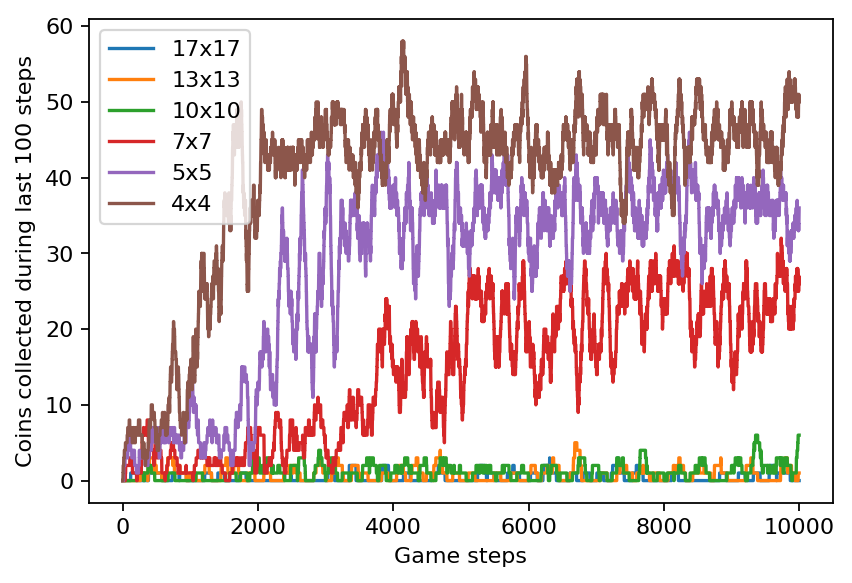
\includegraphics[width=\linewidth]{images/minigame-dense64-arch.png}
    \caption{Dense 64 (\ref{fig:dense-arch64})}
    \label{fig:network-dense64}
  \end{subfigure}
  \quad
  \begin{subfigure}[b]{0.48\linewidth}
    \centering
      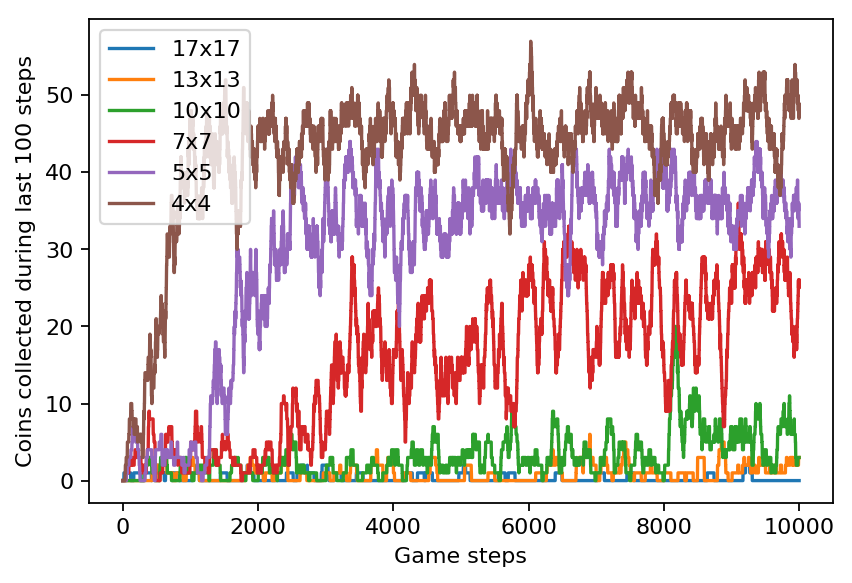
\includegraphics[width=\linewidth]{images/minigame-dense256-arch.png}
    \caption{Dense 256 (\ref{fig:dense-arch256})}
    \label{fig:network-dense256}
  \end{subfigure}
  \begin{subfigure}[b]{0.48\linewidth}
    \centering
    	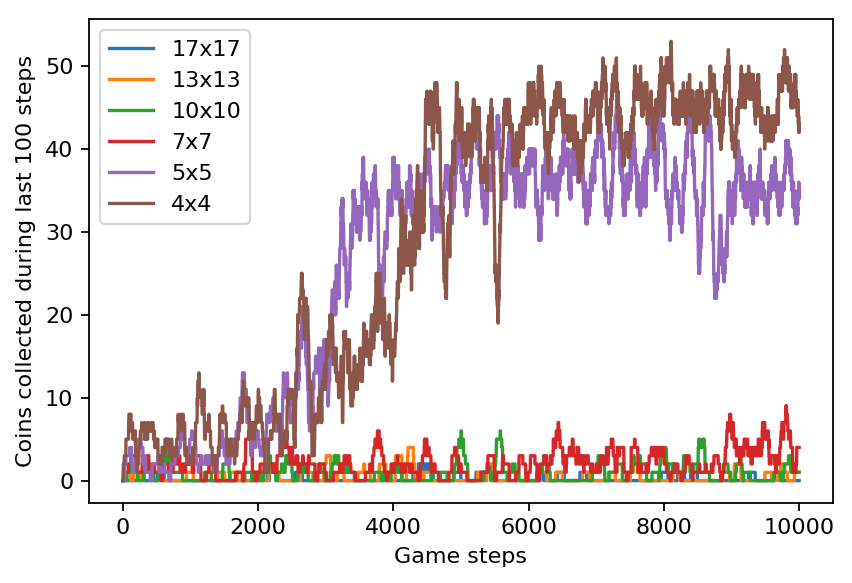
\includegraphics[width=\linewidth]{images/minigame-conv8-4-3-arch.png}
    \caption{Conv from Rainbow paper\cite{Hessel2018RainbowCI} (\ref{fig:conv-original})}
    \label{fig:network-conv843}
  \end{subfigure}
  \quad
  \begin{subfigure}[b]{0.48\linewidth}
    \centering
      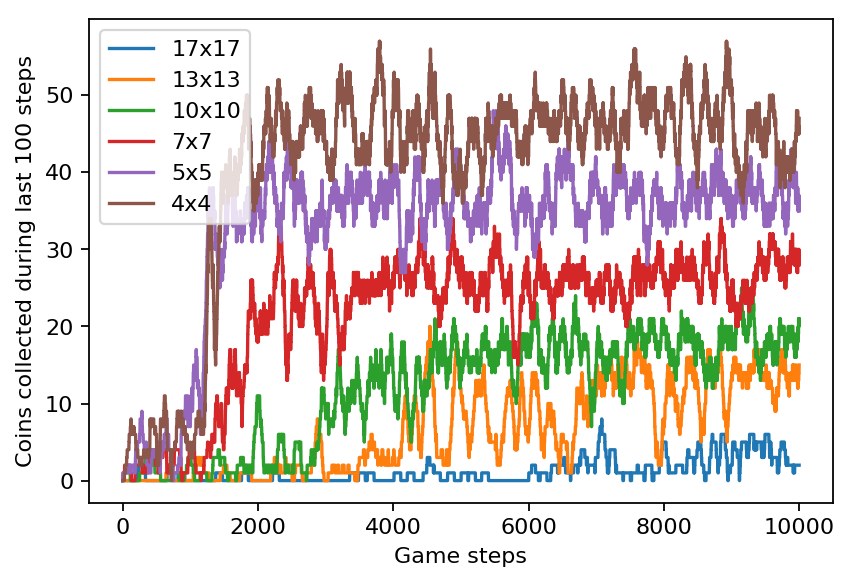
\includegraphics[width=\linewidth]{images/minigame-conv1-4-3-arch.png}
    \caption{Conv modified (\ref{fig:conv-modified})}
    \label{fig:network-conv143}
  \end{subfigure}
  \caption{Agents with different network architectures playing the minigame introduced in \ref{ch:minigame} for arena sizes from $4\times4$ to $17\times17$. There are three coins that can be collected per episode. The graphs show coins collected during the last 100 steps, continuing over episodes. For a big arena this number is naturally lower because of the large distances between coins, but it can be seen when and if the agent is plateauing.}
  \label{fig:networks}
\end{figure}

